\chapter{研究の準備}\label{cha:Preparation}
本章では、本研究で必要となる前提知識を説明する。
% \section{モータ作成}\label{motor}
% \subsection{仕様書}\label{siyo}
% \subsection{シミュレータの役割}\label{simu}
\section{ブラシ付きDCモータ}\label{}
% ブラシ付きDCモータだけかけばいいのか?モータ全体の話も必要か?
ブラシ付きモータとは、ーーー
今回試作するツールでは、ブラシ付きモータのシミュレーション結果に対応する。

\section{対応するモデル}\label{taioumodel}
試作するモータ特性表自動生成ツールでは、以下のModelicaモデルのシミュレーション結果に対応する。
\begin{itemize}
	\item モータ単体のModelicaモデル !!!
	\item モータ単体のModelicaモデルをサブシステムとするモデル
\end{itemize}
以降、上記のモデルについて具体的に説明する。

\subsection{モータ単体のModelicaモデル}\label{sub:tanntai}
!!! モータ単体の話ではなくブラシ付きDCモータの話になっている。
モータ単体のModelicaモデルとは、電源部品、抵抗部品、インダクター部品、起電力部品、慣性部品、接地部品を持つモデルのことである。\\
上記6つの部品が必要な理由は、ブラシ付きDCモータの等価回路\cite{等価回路}をModelica言語で表す際に、使用する部品\cite{modelicaシステム本}だからである。\\
各部品で使用するMSLを表\ref{tab:MSL}に、ブラシ付きDCモータの等価回路を図\ref{fig:touka}に、モータ単体のModelicaモデルの例を図\ref{fig:tantai_model}に、
図\ref{fig:tantai_model}のModelicaコードを図\ref{fig:tantai_modelica}に、それぞれ示す。

\begin{table}[t]
	\centering
	\caption{MSL対応表}
	\begin{tabular}{|c|c|} \hline
	  部品名 & 使用するMSL \\ \hline \hline
	  電源部品 & Modelica.Electrical.Analog.Sources \\ \hline
	  抵抗部品 & Modelica.Electrical.Analog.Basic \\ \hline
	  インダクター部品 & Modelica.Electrical.Analog.Basic \\ \hline
	  起電力部品 & Modelica.Electrical.Analog.Basic \\ \hline
	  慣性部品 & Modelica.Mechanics.Rotational.Components \\ \hline
	  接地部品 & Modelica.Electrical.Analog.Basic \\ \hline
	\end{tabular}
	\label{tab:MSL}
  \end{table}
 
\begin{figure}[t]
	\centering
	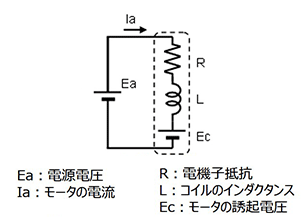
\includegraphics[width=7cm]{./Image/touka.png}
	\caption{ブラシ付きDCモータの等価回路}
	\label{fig:touka}
  \end{figure}

\begin{figure}[t]
  \centering
  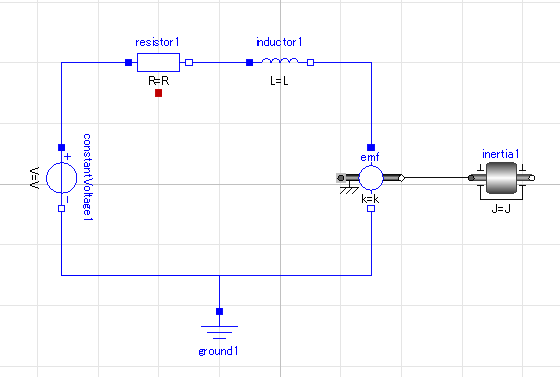
\includegraphics[width=10cm]{./Image/tantai_model.png}
  \caption{モータ単体のModelicaモデルの例}
  \label{fig:tantai_model}
\end{figure}


% \begin{figure*}[t]
% 	\lstinputlisting[label={code:motor}, caption={図\ref{fig:tantai_model}のModelicaコード}]{./chapters/motor.mo}
% \end{figure*}

\begin{figure}[t]
	\centering
	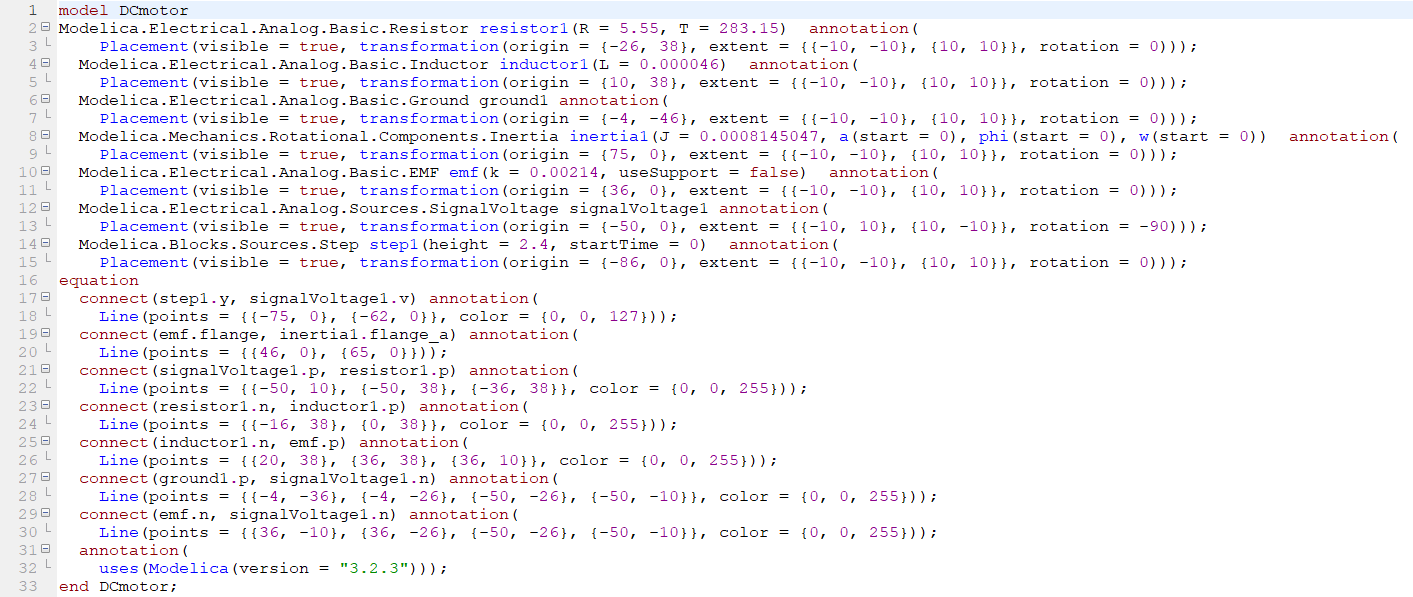
\includegraphics[width=16.5cm,height=8cm]{./Image/tantai_modelica.png}
	\caption{図\ref{fig:tantai_model}のModelicaコード}
	\label{fig:tantai_modelica}
  \end{figure}

%   \vspace{-1zh}

\subsection{モータ単体のModelicaモデルをサブシステムとするモデル} \label{sub:submodel}
モータ単体のModelicaモデルをサブシステム\cite{modelicaシステム本}とするモデルとは、
\ref{sub:tanntai}節で説明したモータ単体のModelicaモデルを1つのサブシステムとして扱い、他の部品と合わせたモデルのことである。\\
例として、DCモータのサブシステムを用いたDCモータサーボのモデルを図\ref{fig:submodel}に、図\ref{fig:submodel}のModelicaコードを図\ref{fig:sub_modelica}に、それぞれ示す。

\begin{figure}[t]
	\centering
	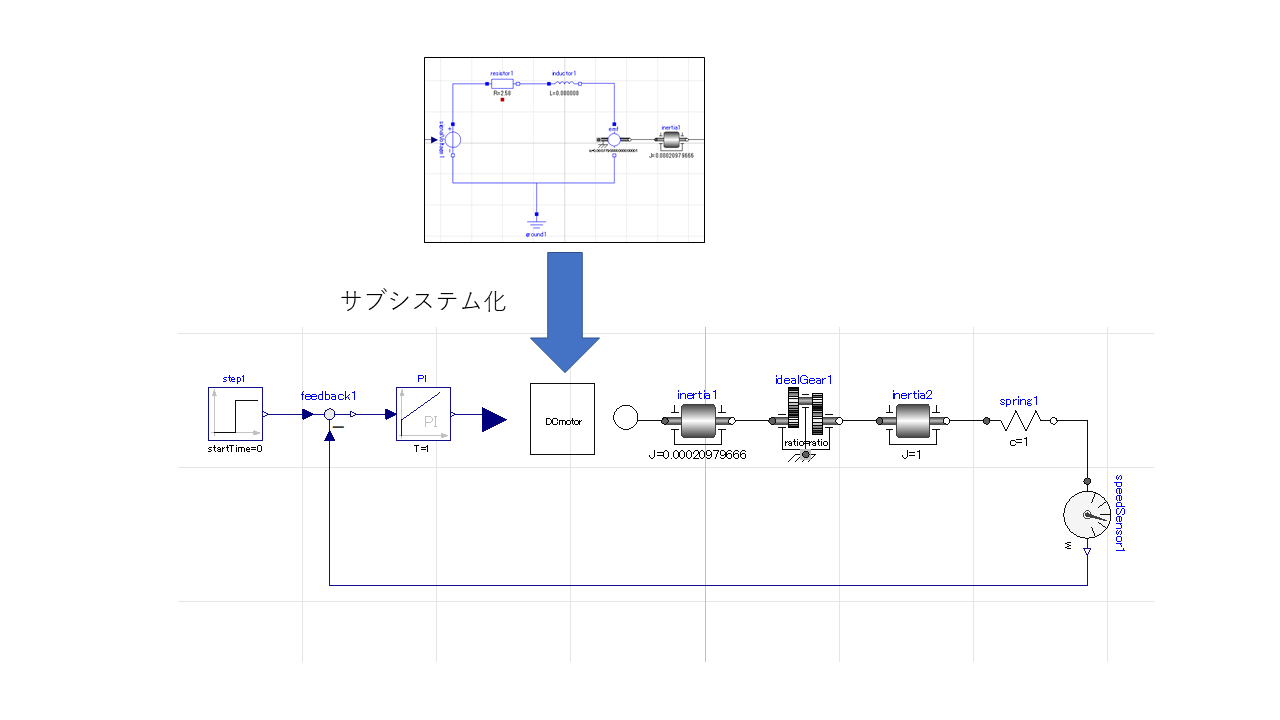
\includegraphics[width=16.5cm,height=10cm]{./Image/submodel_pack.png}
	\caption{DCモータサーボのモデル}
	\label{fig:submodel}
  \end{figure}

  \begin{figure}[t]
	\centering
	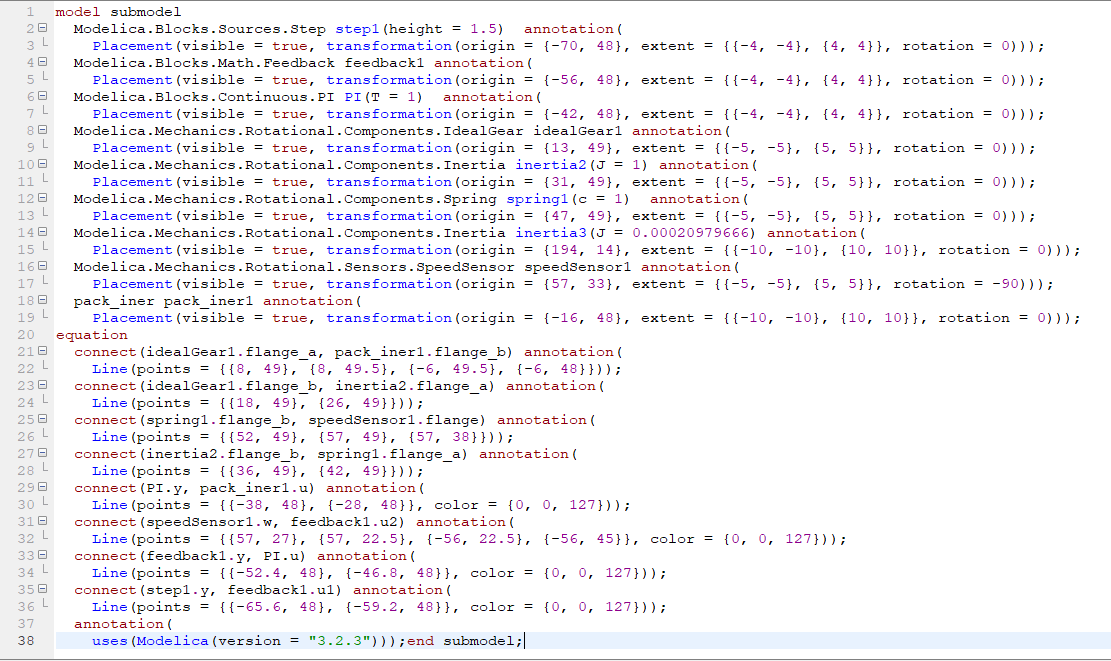
\includegraphics[width=16.5cm,height=10cm]{./Image/sub_modelica.png}
	\caption{図\ref{fig:submodel}のModelicaコード}
	\label{fig:sub_modelica}
  \end{figure}

  \subsection{モデル作成時の制約}\label{sub:seiyaku}
  \ref{sub:tanntai}章、\ref{sub:submodel}章で説明した制約の他に、以下の制約も満たしていなければならない。

  \begin{itemize}
	  \item 入力は0秒スタート
	  \item 電圧値は一定
	  \item 各部品に名前をつける際は、デフォルトの名前にする
	  \item モータのモデルは1つまで
  \end{itemize}


\section{OpenModelica}\label{OM}
Modelica言語に対応したOSSである\cite{fritzson2006openmodelica}。

\subsection{出力}\label{output}
OpenModelicaでは、シミュレーション結果の保存先を、以下の3つの形式から選択することができる。

\begin{itemize}
    \item matファイル
    \item pltファイル
    \item csvファイル
\end{itemize}

csvファイルに書かれている内容について説明!

csvファイルの名前の生成規則について説明!

図\ref{fig:tantai_model}のモデルをシミュレーションした時に、OpenModelicaから出力されるcsvファイルの一部を、図\ref{fig:simyu_csv}に示す。\\


また、OpenModelicaでは、シミュレーション結果を、グラフとして画面上に描画することが可能である。

\subsection{グラフィカルモデリング}\label{glafical}
サブセクションで書くなら何か他にも書く。

\section{Modelica言語}\label{modelica}
微分代数方程式を用いた複合領域の物理システムモデリングのために開発されたオブジェクト指向言語である。\\
 \subsection{Modelica標準ライブラリ(MSL)}\label{MSL}
        Modelica言語による様々な物理領域のモデルライブラリを開発しており、
        数学、機械、電気、熱、流体、制御系、状態遷移機械などを含んだフリーのライブラリがリリースされている。

\section{モータ特性表}\label{mortoku}
モータ特性表とは、モータを選定する際に、参考にする資料である。一般的に決まった形式はなく、各会社によって書いている要素は異なるため、
10社のモータ特性表をもとに、作成するモータ特性表の要素を決定した。\\
以下にモータ特性表の構成と、要素を示す。

% \subsection{特性表}\label{sub:tokuhyou}
% モータを選定する際に、参考にする資料。
% 図?

% \subsection{特性グラフ}\label{sub:tokugura}



  \section{Python}\label{python}
  !!!未調査!!!